\part{Conditioning and Stability}
\chapter{Conditioning and Condition Numbers}

Conditioning pertains to the perturbation behavior of a mathematical problem. Stability pertains to the perturbation behavior of an algorithm used to solve that problem on a computer.

\section{Condition of a Problem} 
In the abstract, we can give the following definition of mathematical problems. 


%────────────────────────────────────────
\begin{definition}
[Problem]
\label{def: Problem}
A mathematical problem is a function $f:X\to Y$ where $X$ is the vector space of data and $Y$ is the vector space of solutions.
\end{definition}
%────────────────────────────────────────


This function $f$ is usually nonlinear (even in linear algebra), but most of the time it is at least continuous.

Typically we shall be concerned with the behavior of a problem $f$ at a particular data point $x \in X$ (the behavior may vary greatly from one point to another). The combination of a problem $f$ with prescribed data $x$ might be called a \textbf{problem instance}, but it is more usual, though occasionally confusing, to use the term \textbf{problem} for this notion too.

A \textbf{well-conditioned} problem (instance) is one with the property that all small perturbations of $x$ lead to only small changes in $f(x)$. An ill-conditioned problem is one with the property that some small perturbation of $x$ leads to a large change in $f(x)$.

\section{Absolute Condition Number} 

%────────────────────────────────────────
\begin{definition}
[Absolute condition number]
\label{def: Absolute condition number}
Let $\delta x$ denote a small perturbation of $x$, and write $\delta f=f(x+\delta x)-f(x)$. The absolute condition number $\hat{\kappa}=\hat{\kappa}(x)$ of the problem $f$ at $x$ is defined as
$$
\hat{\kappa}=\lim _{\delta \rightarrow 0} \sup _{\|\delta x\| \leq \delta} \frac{\|\delta f\|}{\|\delta x\|}
$$
\end{definition}
%────────────────────────────────────────
We can also write this as: 
\[
    \hat{\kappa}=\sup _{\delta x} \frac{\|\delta f\|}{\|\delta x\|}. 
\]
If $f$ is differentiable, we can evaluate the condition number by the Jacobian matrix. Let $J(x)$ be the Jacobian of $f$ at $x$. We have 
\[
    \hat \kappa = \|J(x)\|, 
\]
where $\|J(x)\|$ is the induced norm by the norms on $X$ and $Y$. 

\section{Relative Condition Number} 
When we are concerned with relative changes, we need the notion of relative condition.  


%────────────────────────────────────────
\begin{definition}
[Relative condition number]
\label{def: Relative condition number}
The relative condition number $\kappa=\kappa(x)$ is defined by
$$
\kappa=\lim _{\delta \rightarrow 0} \sup _{\|\delta x\| \leq \delta}\left(\frac{\|\delta f\|}{\|f(x)\|} / \frac{\|\delta x\|}{\|x\|}\right). 
$$
\end{definition}
%────────────────────────────────────────
If $f$ is differentiable, we can express this quantity in terms of the Jacobian: 
\[
    \kappa=\frac{\|J(x)\|}{\|f(x)\| /\|x\|}. 
\]
Both absolute and relative condition numbers have their uses, but the latter are more important in numerical analysis. This is ultimately because the floating point arithmetic used by computers introduces relative errors rather than absolute ones; see the next lecture. A problem is \textbf{well-conditioned} if $\kappa$ is small (e.g., $1,10,10^2$), and \textbf{ill-conditioned} if $\kappa$ is large (e.g., 10 $10^6$).

\begin{example}
\begin{itemize}
    \item []
    \item  Consider the trivial problem of obtaining the scalar $x / 2$ from $x \in \mathbb{C}$. The Jacobian of the function $f: x \mapsto x / 2$ is just the derivative $J=f^{\prime}=1 / 2$, so by (12.6),
    $$
    \kappa=\frac{\|J\|}{\|f(x)\| /\|x\|}=\frac{1 / 2}{(x / 2) / x}=1 .
    $$
    This problem is well-conditioned by any standard.
    \item Consider the problem of computing $\sqrt{x}$ for $x>0$. The Jacobian of $f: x \mapsto \sqrt{x}$ is the derivative $J=f^{\prime}=1 /(2 \sqrt{x})$, so we have
    $$
    \kappa=\frac{\|J\|}{\|f(x)\| /\|x\|}=\frac{1 /(2 \sqrt{x})}{\sqrt{x} / x}=\frac{1}{2} .
    $$
    Again, this is a well-conditioned problem.
    \item Consider the problem of obtaining the scalar $f(x)=x_1-x_2$ from the vector $x=\left(x_1, x_2\right)^* \in \mathbb{C}^2$. For simplicity, we use the $\infty$-norm on the data space $\mathbb{C}^2$. The Jacobian of $f$ is
    $$
    J=\left[\begin{array}{ll}
    \frac{\partial f}{\partial x_1} & \frac{\partial f}{\partial x_2}
    \end{array}\right]=\left[\begin{array}{ll}
    1 & -1
    \end{array}\right]
    $$
    with $\|J\|_{\infty}=2$. The condition number is thus
    $$
    \kappa=\frac{\|J\|_{\infty}}{\|f(x)\| /\|x\|}=\frac{2}{\left|x_1-x_2\right| / \max \left\{\left|x_1\right|,\left|x_2\right|\right\}} .
    $$
    This quantity is large if $\left|x_1-x_2\right| \approx 0$, so the problem is ill-conditioned when $x_1 \approx x_2$, matching our intuition of the hazards of ``cancellation error.''
    \item The problem of computing the eigenvalues of a nonsymmetric matrix is also often ill-conditioned. One can see this by comparing the two matrices
    $$
    \left[\begin{array}{cc}
    1 & 1000 \\
    0 & 1
    \end{array}\right], \quad\left[\begin{array}{cc}
    1 & 1000 \\
    0.001 & 1
    \end{array}\right],
    $$
    whose eigenvalues are $\{1,1\}$ and $\{0,2\}$, respectively. On the other hand, if a matrix $A$ is symmetric (more generally, if it is normal), then its eigenvalues are well-conditioned. It can be shown that if $\lambda$ and $\lambda+\delta \lambda$ are corresponding eigenvalues of $A$ and $A+\delta A$, then $|\delta \lambda| \leq\|\delta A\|_2$, with equality if $\delta A$ is a multiple of the identity. Thus the absolute condition number of the symmetric eigenvalue problem is $\hat{\kappa}=1$, if perturbations are measured in the 2-norm, and the relative condition number is $\kappa=\|A\|_2 /|\lambda|$.
\end{itemize}
\end{example}


%────────────────────────────────────────
\begin{example}
[Root of Polynomial]
\label{eg: Root of Polynomial}
The determination of the roots of a polynomial, given the coefficients, is a classic example of an ill-conditioned problem. Assume we have a polynomial $p(x) = \sum_{i=0}^n a_i x^i$. If the ith coefficient $a_i$ is pertubed by infinitesimal quantity $\delta  a_i$, the perturbation of the $j$th root $x_j$ satisfies: 
\[
    \sum_{k \neq i} a_k (x_j + \delta  x_j)^k + (a_i+ \delta a_i) (x_j + \delta  x_j)^i = 0 \Rightarrow \delta a_i x_j^i + \sum_k k a_k x_j^{k-1} \delta x_j= 0. 
\]
Hence, $ \delta x_j = \frac{(\delta a_i) x_j^i}{p'(x_j) }. $  So the condition number of $x_j$ w.r.t. perturbations of $a_i$ is: 
\[
    \kappa = \frac{|\delta x_j|}{|x_j|}/ \frac{|\delta  a_i|}{|a_i|} = \frac{|a_i x_j^{i-1}|}{|p'(x_j)|}. 
\]
This number can be very large. If we consider the ``Wilkinson polynomial'', 
\[
    p(x) = \prod_{i=1}^20 (x-i) = a_0 + a_1 x + \cdots + a_{19} x^{19} + x^{20}.  
\]

%────────────────────────────────────────
\begin{figure}[H]
    \centering
    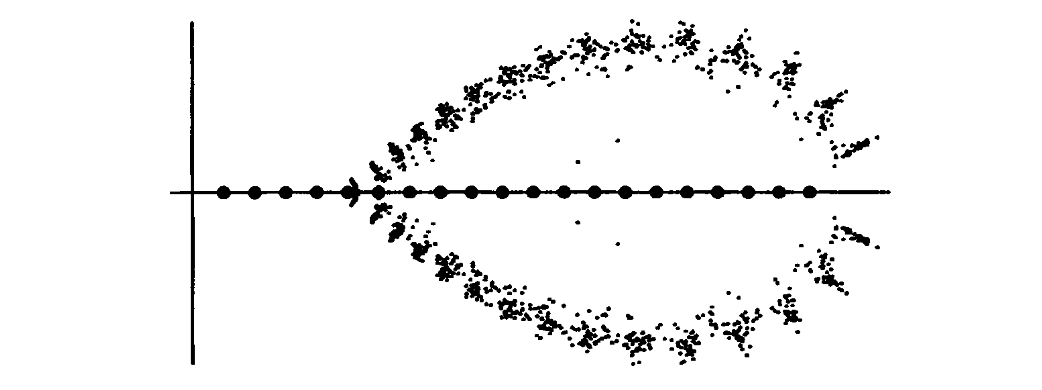
\includegraphics[width=0.8\textwidth]{figures/12-1.png}
    \label{fig: wikinson} 
    \caption{Wilkinson's classic example of ill-conditioning. The large dots are the roots of the unperturbed polynomial. The samll dots are the super imposed roots in the complex plane of 100 randomly perturbed polynomials with coefficients defined by $\overline{a_k} = a_k ( 1+ 10^{-10}r_k)$, where $r_k\sim \cN(0,1)$. }
\end{figure}
%────────────────────────────────────────

The most sensitive root of this polynomial is $x=15$, and it's most sensitive in the coefficient $a_{15} \approx 1.67\times 10^9$. The condition number is: 
\[
    \kappa \approx \frac{1.67\times 10^8 \cdot 15^14}{5!14!} \approx 5.1 \times 10^{13}.
\]
\end{example}
%────────────────────────────────────────


\section{Condition of Matrix-Vector Multiplication} 
Given $A\in \CC^{m\times n}$ and consider the problem of computing $Ax$ is 
\[
    \kappa=\sup _{\delta x}\left(\frac{\|A(x+\delta x)-A x\|}{\|A x\|} / \frac{\|\delta x\|}{\|x\|}\right)=\sup _{\delta x} \frac{\|A \delta x\|}{\|\delta x\|} / \frac{\|A x\|}{\|x\|} = \|A\| \frac{\|x\|}{\|Ax\|}.  
\]

Then we can use the fact that $\|x\|/ \|Ax\| \le \|A^{-1}\|$ to loosen to a bound independent of $x$: 
\[
    \kappa \leq\|A\|\left\|A^{-1}\right\| .
\]
In fact, $A$ need not have been square. If $A\in \CC^{m\times n}$ with $m\ge n$ has full rank, we can replace $A^{-1}$ by the pseudoinverse $A^\dagger $. 


%────────────────────────────────────────
\begin{theorem}
\label{thm: condition number of A}
Let $A \in \mathbb{C}^{m \times m}$ be nonsingular and consider the equation $A x=b$. The problem of computing $b$, given $x$, has condition number
\begin{equation}
    \label{eq: cond of A}
    \kappa=\|A\| \frac{\|x\|}{\|b\|} \leq\|A\|\left\|A^{-1}\right\|
\end{equation}
with respect to perturbations of $x$. The problem of computing $x$, given $b$, has condition number
\begin{equation}
    \label{eq: cond of Ainv}
    \kappa=\left\|A^{-1}\right\| \frac{\|b\|}{\|x\|} \leq\|A\|\left\|A^{-1}\right\|    
\end{equation}
with respect to perturbations of $b$. If $\|\cdot\|=\|\cdot\|_2$, then equality holds in the first inequality if $x$ is a multiple of a right singular vector of $A$ corresponding to the minimal singular value $\sigma_m$, and equality holds in the second inequality if $b$ is a multiple of a left singular vector of $A$ corresponding to the maximal singular value $\sigma_1$.
\end{theorem}
%────────────────────────────────────────

\section{Condition Number of a Matrix}  
The product $\|A\|\left\|A^{-1}\right\|$ comes up so often that it has its own name: 

%────────────────────────────────────────
\begin{definition}
[Condition number of matrix]
\label{def: Condition number of matrix}
The condition number of a mtrix $A\in \CC^{n\times n}$ denoted by $\kappa(A)$: 
\[
    \kappa(A)=\|A\|\left\|A^{-1}\right\| .
\]
\end{definition}
%────────────────────────────────────────

If $\kappa(A)$ is small, $A$ is said to be \textbf{well-conditioned}; if $\kappa(A)$ is large, $A$ is \textbf{ill-conditioned}. If $A$ is singular, it is customary to write $\kappa(A)=\infty$. Note that if $\|\cdot\|=\|\cdot\|_2$, then $\|A\|=\sigma_1$ and $\left\|A^{-1}\right\|=1 / \sigma_m$. Thus
$$
\kappa(A)=\frac{\sigma_1}{\sigma_m}
$$
in the 2-norm, and it is this formula that is generally used for computing $2-$norm condition numbers of matrices. 

For a rectangular matrix $A \in \mathbb{C}^{m \times n}$ of full rank, $m \geq n$, the condition number is defined in terms of the pseudoinverse: $\kappa(A)=\|A\|\left\|A^{+}\right\|$. Since $A^{+}$ is motivated by least squares problems, this definition is most useful in the case $\|\cdot\|=\|\cdot\|_2$, where we have
$$
\kappa(A)=\frac{\sigma_1}{\sigma_n}. 
$$

\section{Condition of a System of Equations} 

In Theorem~\ref{thm: condition number of A} , we held $A$ fixed and perturbed $x$ or $b$. What happens if we perturb $A$ ? Specifically, let us hold $b$ fixed and consider the behavior of the problem $A \mapsto x=A^{-1} b$ when $A$ is perturbed by infinitesimal $\delta A$. Then $x$ must change by infinitesimal $\delta x$, where
$$
(A+\delta A)(x+\delta x)=b .
$$
Using the equality $A x=b$ and dropping the doubly infinitesimal term $(\delta A)(\delta x)$, we obtain $(\delta A) x+A(\delta x)=0$, that is, $\delta x=-A^{-1}(\delta A) x$. This equation implies $\|\delta x\| \leq\left\|A^{-1}\right\|\|\delta A\|\|x\|$, or equivalently,
$$
\frac{\|\delta x\|}{\|x\|} / \frac{\|\delta A\|}{\|A\|} \leq\left\|A^{-1}\right\|\|A\|=\kappa(A) \text {. }
$$
Equality in this bound will hold whenever $\delta A$ is such that
$$
\left\|A^{-1}(\delta A) x\right\|=\left\|A^{-1}\right\|\|\delta A\|\|x\|,
$$
and it can be shown by the use of dual norms that for any $A$ and $b$ and norm $\|\cdot\|$, such perturbations $\delta A$ exist. This leads us to the following result.


%────────────────────────────────────────
\begin{theorem}
\label{thm: condition of Ainvb}
Let $b$ be fixed and consider the problem of computing $x=$ $A^{-1} b$, where $A$ is square and nonsingular. The condition number of this problem with respect to perturbations in $A$ is
\begin{equation}
    \label{eq: cond of purturb A}
    \kappa=\|A\|\left\|A^{-1}\right\|=\kappa(A) .
\end{equation}
\end{theorem}
%────────────────────────────────────────


%────────────────────────────────────────
\begin{note}
    Theorems~\ref{thm: condition number of A} and \ref{thm: condition of Ainvb} are of fundamental importance in numerical linear algebra, for they determine how accurately one can solve systems of equations. If a problem $A x=b$ contains an ill-conditioned matrix $A$, one must always expect to ``lose $\log _{10} \kappa(A)$ digits'' in computing the solution, except under very special circumstances. 
\end{note}
%────────────────────────────────────────
